%label:"art:tropicalZeroSet"
%type:"article"
%name:"the zero locus of a tropical polynomial"


The next question is to understand the zero set of a tropical function.  When $f$ is a polynomial, we have the associated variety $V(f):= \{q\st f(q)=0\}$. Na\"ively, one might try define the tropical zero set to be the set where $\TropB(f)=-\infty$ (as $-\infty$ is the tropical additive identity). However, it is clear to see that this will have no solutions. 
%label:"exm:tropicalamoeba"
%type:"example"
%name:"tropical amoeba"


    Take $f=q_1+q_2+1$, where $q_1,q_2 \in (\CC^*)^2$. Drawing the image of $V(f)$ under $\Log_t$ gives us the following sequence of images:
\begin{figure}

\end{figure}
    We call the image of $V(f)$ under the $\Log_t$ map the \emph{amoeba} of $V(f)$, which (in this example) appears to converge to some piecewise linear object.


This mimics the following behavior. A tropical polynomial $\phi: \RR^n\to \RR$ by definition, is a convex piecewise integral affine function on $\RR^2$. We can associate to every such function the locus where $\phi$ where $\phi$ is not differentiable. This will be a union of polyhedra of dimension $n-1$.
%label:"def:tropicalzeroset"
%type:"definition"
%name:"tropical zero set"


    Let $\phi: \RR^n\to \RR$ be a tropical polynomial. The \emph{tropical zero set} is set 
    \[V(f):=\{q\in \RR^n \text{ such that $f$ is not differentiable at $q$}\}.\]





We now give some more details to the previous section. 
%label:"def:integralaffinefunction"
%type:"definition"
%name:"integral affine function"


    Fix a lattice structure $\ZZ^n\subset \RR^n$ and $\ZZ\subset \RR$. 
    We say that a function $\underline \phi: \RR^n\to \RR$ is \emph{integral affine} if $\underline \phi= \phi_{l}+c$ where $\phi_{l}$ is $\ZZ$-linear and $c\in \RR$ is some constant. 


%label:"def:affinehalfspace"
%type:"definition"
%name:"affine halfspace"


    For $\underline \phi: \RR^n\to \RR$ a integral affine structure, define $H_{\underline \phi}:= \{q\in \RR^n \st \underline\phi(q) \geq 0 \}.$


%label:"def:rationalpolyhedron"
%type:"definition"
%name:"rational polyhedron"


    We say that $\sigma\subset \RR^n$ is a \emph{rational polyhedron} if $\sigma = \bigcap_{i\in I} H_{\underline \phi_i}$ for some collection of integral affine functions.
    \begin{itemize}
        \item We say that it is a cone  if a translate of it is closed under multiplication by $\RR_{\geq 0}$
        \item We say that $\sigma$ is a polytope if it is compact. 
    \end{itemize}


%label:"def:polyhedralcomplex"
%type:"definition"
%name:"polyhedral complex"


    A set of polyhedra is called a \emph{polyhedral complex} if
    \begin{itemize}
        \item if $\sigma\in P$, then every face $\tau< \sigma$ is also contained in $P$,
        \item For $\sigma_1, \sigma_2\in P$: if $\sigma_1\cap\sigma_2= \tau \neq \emptyset$,then $\tau$ is a face of both $\sigma$ and $\sigma'$. 
    \end{itemize}


%label:"fig:somePolyhedralComplexes"
%author:JeffHicks
%name:"examples and nonexamples of polyhedral complexes."
%type:"figure"
%parent:"con:dehnTwist"
%caption:"Two examples of unions of polyhedra. On the left, a polyhedral complex. The right figure is not an example of a polyhedral complex"

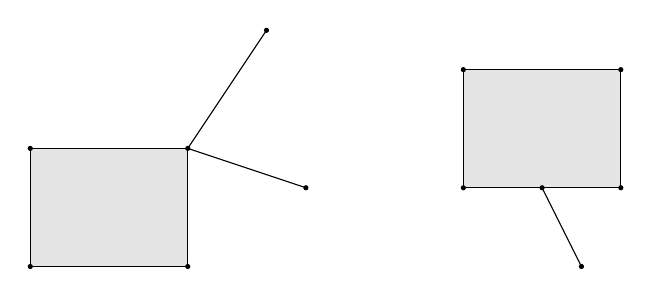
\begin{tikzpicture}\begin{scope}[]

    \draw (-1,1.5) -- (-2,0) -- (-0.5,-0.5);
    \draw[fill=gray!20]  (-4,-1.5) rectangle (-2,0);
\end{scope}\begin{scope}[shift={(5.5,1)}]

    \draw[fill=gray!20]  (-4,-1.5) rectangle (-2,0);
    \draw (-3,-1.5) -- (-2.5,-2.5);
\end{scope}
\node[fill=black, circle, scale=.2] at (-4,-1.5) {};
\node[fill=black, circle, scale=.2] at (-4,0) {};
\node[fill=black, circle, scale=.2] at (-2,0) {};
\node[fill=black, circle, scale=.2] at (-2,-1.5) {};
\node[fill=black, circle, scale=.2] at (-0.5,-0.5) {};
\node[fill=black, circle, scale=.2] at (-1,1.5) {};
\node[fill=black, circle, scale=.2] at (1.5,-0.5) {};
\node[fill=black, circle, scale=.2] at (2.5,-0.5) {};
\node[fill=black, circle, scale=.2] at (1.5,1) {};
\node[fill=black, circle, scale=.2] at (3.5,1) {};
\node[fill=black, circle, scale=.2] at (3.5,-0.5) {};
\node[fill=black, circle, scale=.2] at (3,-1.5) {};
\end{tikzpicture}


%label:"lem:polyhedralsubdivision"
%type:"lemma"
%name:"polyhedral subdivision"


    Every set of polyhedra has a polyhedral complex subdivision. 


Later, we will impose some additional criteria on these complexes:
\begin{itemize}
    \item Pure dimension $k$ --- every maximal cell is of dimension $k$,
    \item ``Weighted'': there exists a weight function $\wt: \{\text{Maximal Cells}\} \to \ZZ$
    \item ``Balanced'': for a weighted pure complex: every codimension 1 face $\tau$ is we have $\sum_{\sigma} \wt(\sigma) v_{\sigma/\tau}=0$ in $\RR^n /\span(\tau)$.
\end{itemize}
%label:"def:tropicalkcycle"
%type:"definition"
%name:"tropical k cycle"


    A \emph{tropical $k$-cycle} in $\RR^n$ is a balanced weighted polyhedral complex. 


